\documentclass{article}

% if you need to pass options to natbib, use, e.g.:
% \PassOptionsToPackage{numbers, compress}{natbib}
% before loading nips_2016
%
% to avoid loading the natbib package, add option nonatbib:
% \usepackage[nonatbib]{nips_2016}

%\usepackage{nips_2016}

% to compile a camera-ready version, add the [final] option, e.g.:
\usepackage[final]{nips_2016}

\usepackage[utf8]{inputenc} % allow utf-8 input
\usepackage[T1]{fontenc}    % use 8-bit T1 fonts
\usepackage{hyperref}       % hyperlinks
\usepackage{url}            % simple URL typesetting
\usepackage{booktabs}       % professional-quality tables
\usepackage{amsfonts}       % blackboard math symbols
\usepackage{nicefrac}       % compact symbols for 1/2, etc.
\usepackage{microtype}      % microtypography
\usepackage{graphicx}

\title{Project Proposal: Collaborative Policy Learning for Vehicle Navigation}

% The \author macro works with any number of authors. There are two
% commands used to separate the names and addresses of multiple
% authors: \And and \AND.
%
% Using \And between authors leaves it to LaTeX to determine where to
% break the lines. Using \AND forces a line break at that point. So,
% if LaTeX puts 3 of 4 authors names on the first line, and the last
% on the second line, try using \AND instead of \And before the third
% author name.

\author{
    Chris Ying \\
      Machine Learning Department \\
        Carnegie Mellon University\\
          Pittsburgh, PA 15213 \\
            \texttt{cying@andrew.cmu.edu} \\
              %% examples of more authors
                \And
                  Ananya Kumar \\
                    School of Computer Science \\
                      Carnegie Mellon University \\
                        \texttt{ananyak@andrew.cmu.edu} \\
                          \AND
                            Dominick DiRenzo \\
                              School of Computer Science  \\
                                Carnegie Mellon University \\
                                  Pittsburgh, PA 15213 \\
                                    \texttt{ddirenzo@andrew.cmu.edu} \\
                                      %% \And
                                        %% Coauthor \\
                                          %% Affiliation \\
                                            %% Address \\
                                              %% \texttt{email} \\
                                                %% \And
                                                  %% Coauthor \\
                                                    %% Affiliation \\
                                                      %% Address \\
                                                        %% \texttt{email} \\
}

\begin{document}
% \nipsfinalcopy is no longer used

\maketitle

\section{Overview}

Many recent advances in reinforcement learning have focused on single-agent (e.g. Atari \cite{DBLP:journals/corr/MnihKSGAWR13}) or competitive (e.g. Go \cite{silver2016mastering}) environments. We will explore the task of learning a single policy that controls multiple agents collaborating to complete a task. For a real-world example, consider autonomous vehicles: each vehicle will be running the same code so they all share the same policy and have to "collaborate" to avoid collisions while also getting to the destination.

\begin{figure}[h!]
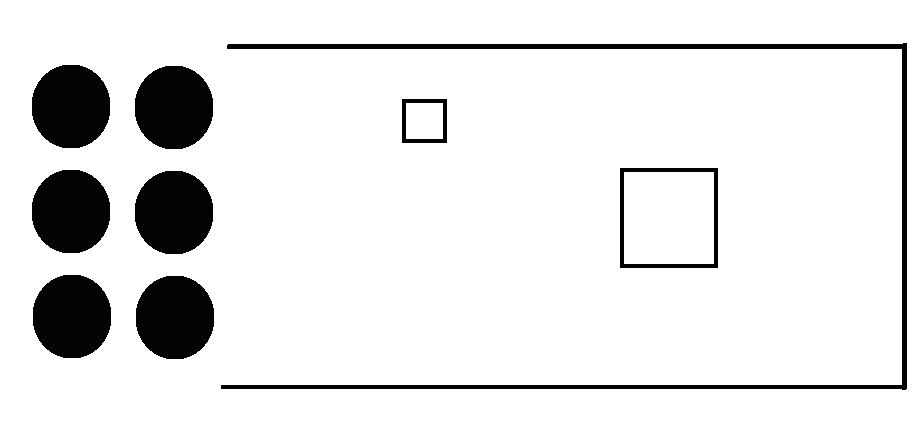
\includegraphics[scale=0.25]{coop_game}
\centering
\caption{Cars are the shaded black circles, end of lane is on the right, rectangles are objects}
\label{fig:coop_game}
\end{figure}

\textbf{Environment} We simulate a group of cars trying to drive across a road lane with a randomly generated obstacle (see figure~\ref{fig:coop_game}). Let $c_i$ be the time it takes car $i$ to reach the end of the road, the goal is to minimize the sum of $c_i$. The cars are identical and circular. The time steps are small discrete steps. Each time step, each car can accelerate in any direction (within imposed limits). Importantly, all the cars must act under the same policy. Each car will only be able to see a local rectangular region of the map. A car's state consists of frames of the local area for the last $n$ steps, and the current velocity and direction. We will have a negative reward for collisions between cars and a positive reward for reaching the destination quickly.

\textbf{Learning} We will use a policy gradient approach. We will set up a neural net that takes in the last few frames of the local map, the current velocity and direction. Based on this input, the neural net needs to output a distribution over possible actions. We will use a Gaussian parametrization, that is, the neural net will output $\mu_v$, $\sigma_d$, which are the mean and standard deviation of a Gaussian distribution, and we will sample the velocity from this distribution, and similarly for the car direction (mod $2\pi$). The neural net architecture will involve a CNN, which takes in the local map frames. This feeds into a few fully connected layers, which takes the CNN, and the current velocity and direction of the car, as input. To train this policy network, we will use a policy gradient approach, such as REINFORCE.

\textbf{Testing} For now, we will fix the size of the lane, and add a single fixed size obstacle at a random location. There will always be a way for all the cars to get to the end of the road. When training, we will generate a random map based on this specification, and run an episode, applying REINFORCE to train. To measure test performance, we will save our final policy, generate random maps, and compute the average performance on the generated maps.

\section{Literature Review}

We plan on using the policy gradient methods discussed in class. For this
we will use the course lecture notes as well as Sutton and Barto's book\cite{sutton1998reinforcement}.
We will be dealing with continuous action spaces so section 13.7 will be useful in particular.

There has been some recent work on multi-agent cooperation, however most of it focuses on 2 agents. We may be able to extend the ideas to a larger number of agents. A recent paper from DeepMind\cite{leibo2017multi} applies reinforcement learning to cooperative 2 player games involving fruit gathering and hunting in a wolfpack. Another paper from Tampuu, Matiisen, et al\cite{tampuu2015multiagent} studies cooperative 2-player pong, where they attempt to make a game last as long as possible.

Ming Tan's old but highly cited paper\cite{tan1993multi} on cooperative learning outlines methodology and results that we can apply to our project.
\section{Project Plan}

By the second milestone we hope to have:
\begin{itemize}
    \item The simulation environment written in OpenAI Gym.
        \item A basic convolutional network set up in Tensorflow for learning the policy function.
            \item A framework to train the policy network via policy gradients.
            \end{itemize}

            By the end of the project we hope to have:
            \begin{itemize}
                \item A fine-tuned policy network for the task.
                    \item A decent training framework that primarily uses policy gradients but may use some supervised learning if necessary for early training.
                        \item Some high-level theoretical explanations of any phenomenon we may observe.
                        \end{itemize}

                        \section{Computational Resources}

                        The most computationally expensive part of our project is the evaluation of the convolutional policy network. Ideally we would like to have a decent GPU (K20 or better) for maybe 1 week of total computation time (conservative estimate).

                        \bibliographystyle{abbrv}
                        \bibliography{bib}

                        \end{document}
